\begin{ex}
(Mackenzie) Cada um dos círculos da figura deverá ser pintado de uma cor, escolhida dentre 4 possíveis. Sabendo que 2 círculos consecutivos nunca serão pintados com a mesma cor, então o número de formas de pintar os círculos é:
\begin{center}
    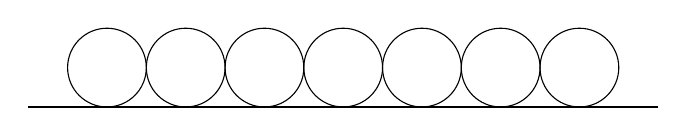
\begin{tikzpicture}
    \draw (-1,0)--(7,0);
    \draw  (0,.5) circle (.5);
    \draw  (1,.5) circle (.5);
    \draw  (2,.5) circle (.5);
    \draw  (3,.5) circle (.5);
    \draw  (4,.5) circle (.5);
    \draw  (5,.5) circle (.5);
    \draw  (6,.5) circle (.5);
    \end{tikzpicture}
\end{center}
   \begin{enumerate}[(a)]
   \item $7^4$
   \item $7!\cdot 4!$
   \item $3 \cdot 7!$
   \item $4^7$
   \item 2916
   \end{enumerate}
     \begin{sol}
      resposta: e \\
      $4\cdot3^6=2916$
     \end{sol}
\end{ex}